\documentclass{standalone}


\usepackage{tikz}
\usetikzlibrary{arrows}

\begin{document}
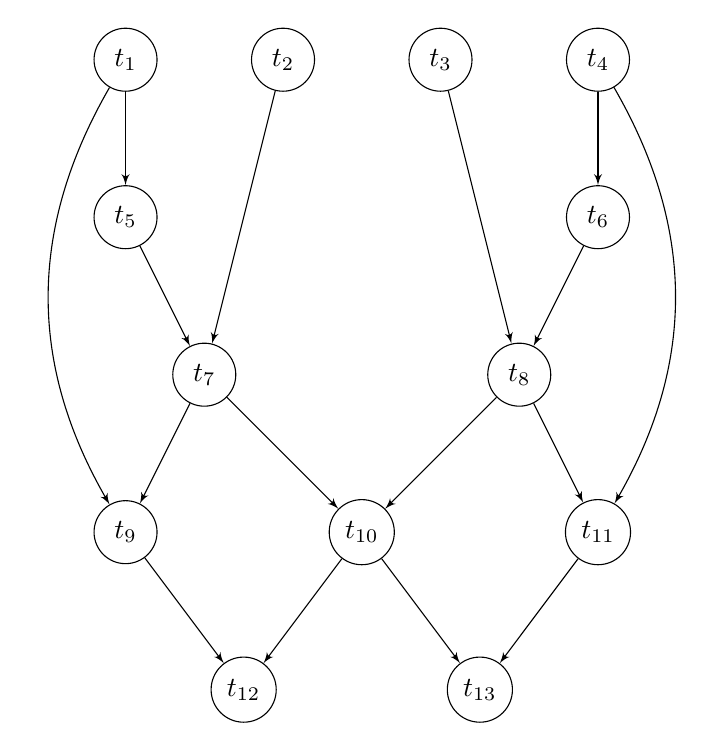
\begin{tikzpicture}[auto, node distance=2cm,>=latex']
\node[circle,draw,minimum size=.8cm] (t1) {$t_1$};
\node[circle,draw,minimum size=.8cm,right of = t1] (t2) {$t_2$};
\node[circle,draw,minimum size=.8cm,right of = t2] (t3) {$t_3$};
\node[circle,draw,minimum size=.8cm,right of = t3] (t4) {$t_4$};
\node[circle,draw,minimum size=.8cm,below of = t1] (t5) {$t_5$};
\node[circle,draw,minimum size=.8cm,below of = t4] (t6) {$t_6$};
\node[circle,draw,minimum size=.8cm,below of = t5,xshift=1cm] (t7) {$t_7$};
\node[circle,draw,minimum size=.8cm,below of = t6,xshift=-1cm] (t8) {$t_8$};
\node[circle,draw,minimum size=.8cm,below of = t7,xshift=-1cm] (t9) {$t_9$};
\node[circle,draw,minimum size=.8cm,below of = t7,xshift=2cm] (t10) {$t_{10}$};
\node[circle,draw,minimum size=.8cm,below of = t8,xshift=1cm] (t11) {$t_{11}$};
\node[circle,draw,minimum size=.8cm,below of = t10,xshift=-1.5cm] (t12) {$t_{12}$};
\node[circle,draw,minimum size=.8cm,below of = t10,xshift=1.5cm] (t13) {$t_{13}$};


\draw [->] (t1) -- (t5);
\draw [->] (t2) -- (t7);
\draw [->] (t3) -- (t8);
\draw [->] (t4) -- (t6);
\draw [->] (t5) -- (t7);
\draw [->] (t6) -- (t8);
\draw [->] (t7) -- (t9);
\draw [->] (t7) -- (t10);
\draw [->] (t8) -- (t10);
\draw [->] (t8) -- (t11);
\draw [->] (t10) -- (t12);
\draw [->] (t10) -- (t13);
\draw [->] (t9) -- (t12);
\draw [->] (t11) -- (t13);
\path (t4) edge[->,bend left] (t11);
\path (t1) edge[->,bend right] (t9);
    %
\end{tikzpicture}

\end{document}